
\section{Debugging and Profiling}
In sequential programming measuring the performance of a program can be done through measuring its execution time.
This can be achieved by recording the time when the program starts and when it finishes and calculating the difference.

However, in concurrent processing, the execution times of individual instructions may overlap, making it challenging to calculate the execution time of the individual instructions \cite[21]{volkovLatencyHiding2016}.

Two commonly used metrics for measuring the performance of concurrent programs are throughput and latency.
Latency refers to the average time taken between the start and end of a task, while throughput represents the amount of work performed per unit of time \cite[21-23]{volkovLatencyHiding2016}.

Following is a selection of tools and methods that have been used for debugging and profiling the programs presented in this thesis.

\subsubsection{Python Profilers}
While none of the following profiling methods offer a complete insight into the performance of asynchronous \py programs, they are useful for identifying bottlenecks and frequently scheduled coroutines.

The built-in Python profiler, \code{CProfile}, can be used to measure the execution time of individual functions and the number of times they are called \cite{pythonsoftwarefoundationPythonProfilers}.
It is particularly helpful in identifying slow-running functions, and visualization tools like \code{SnakeViz} can be used to analyze the collected information \cite{davisSnakeViz2023}.
Another valuable tool is the \code{line_profiler} package, which provides a line-by-line profiler for identifying slow lines of code \cite{kernLineProfilerKernprof2023}.

Other tools, such as the \code{austin} plugin for \gls{vscode}, were tested but ultimately discarded as they did not perform as effectively as the previous two methods \cite{tornettaAustinVSCode2023}.

\subsection{Nsight}
Nsight is a suite of tools for debugging and profiling CUDA applications.
Three tools have been used for debugging and profiling during the \gls{cuda} code presented in Chapter \ref{chap:debayer}.
The \code{Nsight for Visual Studio} plugin for \gls{vscode} enables the use of breakpoints and step-by-step debugging in \gls{cuda} kernels \cite{nvidiaNsightVisualStudio2021}.
As \gls{cuda} code is executed in parallel, this does not always offer the same level of insight as when debugging sequential code, but it can still be useful for identifying errors in the code.

For profiling, the \code{nsys profile} command line tool has been used.
It can be used to collect a wide range of information about the execution of a program, including the execution time of individual kernels and memory transaction times \footnote{On the \jx, profiling Pinned Memory appears to be broken.}, memory usage,
and the number of times each \gls{cuda}-related function is called \cite{nvidiaNVIDIANsightSystems2023}.

The \code{nsys profile} tool can also export the collected information to a \code{sqlite} database, which can be visualized using the \code{Nsight Compute} \gls{gui} \cite{nvidiaNVIDIANsightSystems2023}.
Figure \ref{fig:nsight_timeline} shows a zoomed-out timeline view.

\begin{figure}[H]
    \centering
    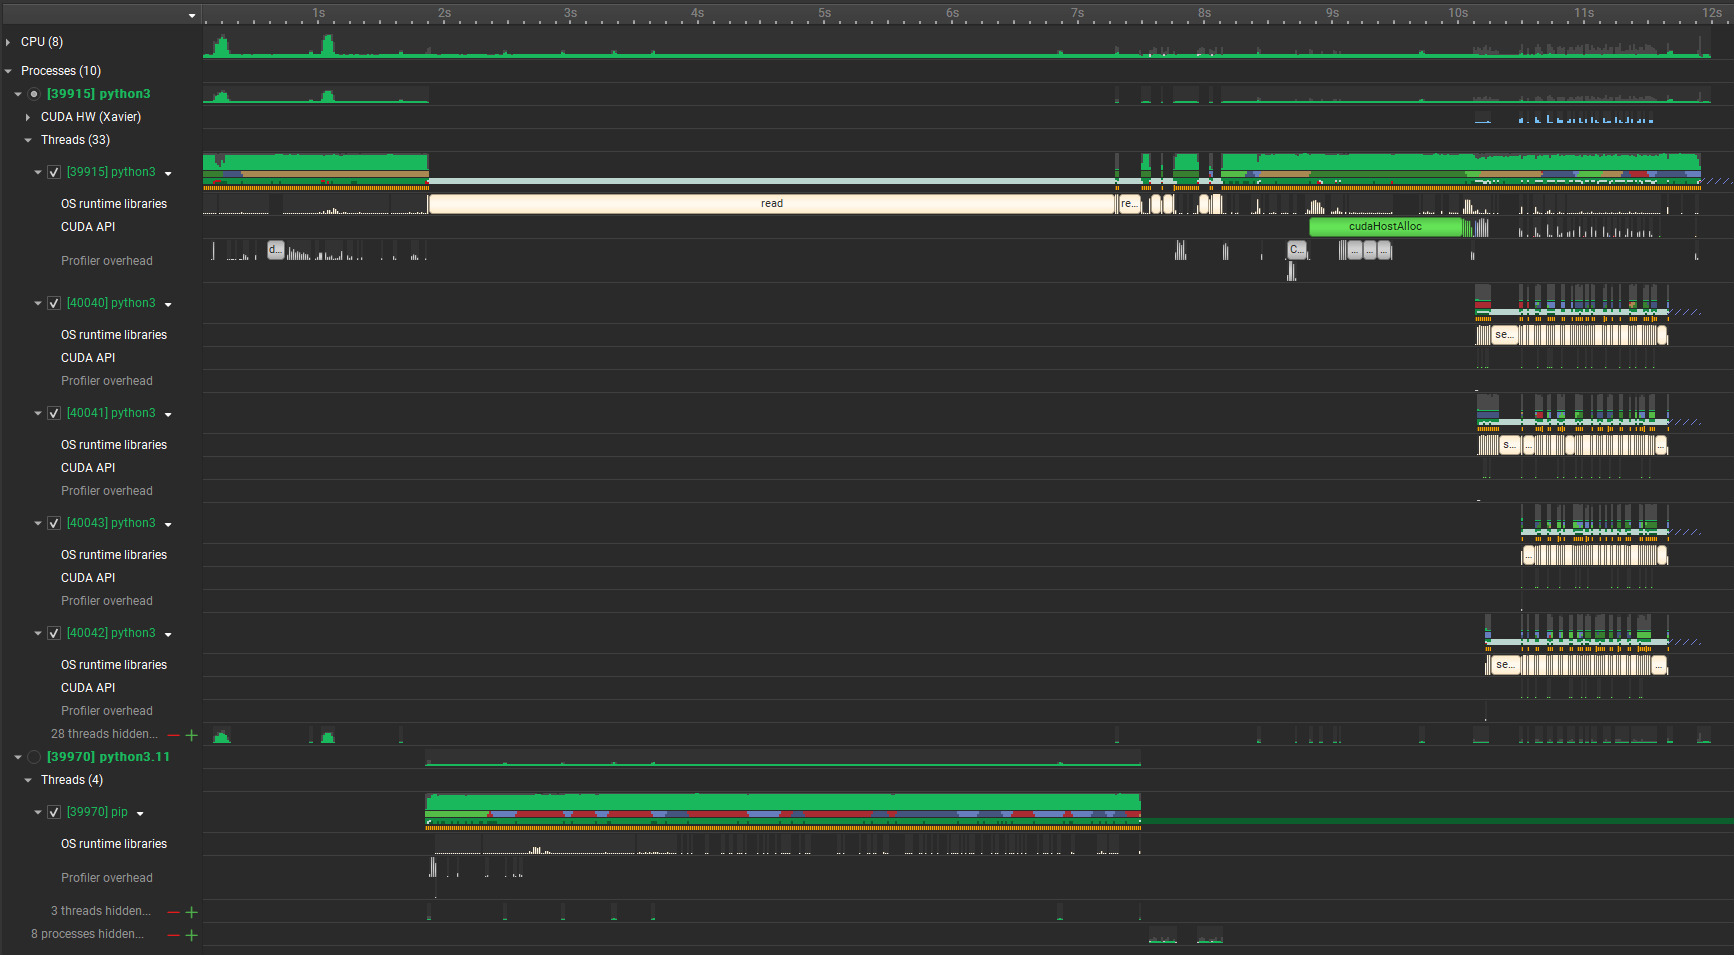
\includegraphics[width=\textwidth]{figures/cuda/nsys_overall.png}
    \caption{Screenshot of Nsight Compute visualizing the profiling of the kernel presented in Chapter \ref{chap:debayer}.}
    \label{fig:nsight_timeline}
\end{figure}

\subsection{Minimal Testing Example and Resource Consumption}
While debugging and profiling the programs presented in this thesis, it was often useful to create a minimal example for profiling elements in isolation.
An example is this is the code used to check the performance difference between threads and coroutines in Listing \ref{listing:concurrency_test}.

This makes it possible to test different implementations and configurations without having to run the entire program and makes it possible to evaluate the resource consumption of individual elements using the \code{jtop} util presented in Section 6.4.4 of the \preproject.

